\documentclass[tikz,border=10pt]{standalone}
\begin{document}

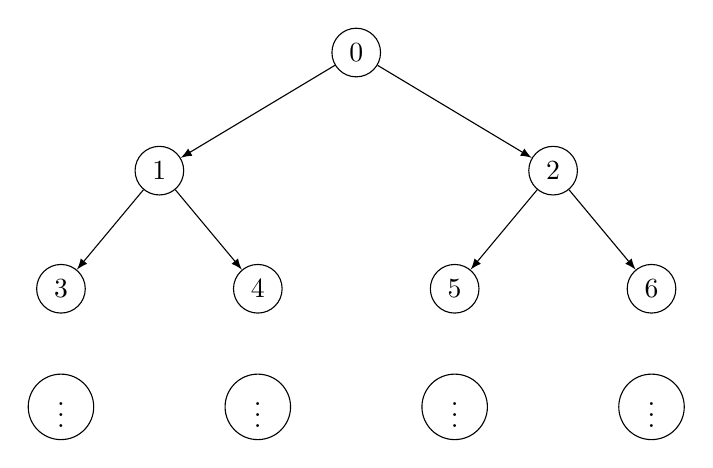
\begin{tikzpicture}[
  level 1/.style={sibling distance=50mm},
  level 2/.style={sibling distance=25mm},
  every node/.style={circle, draw},
  edge from parent/.style={draw, -latex}
]

\node {0}
  child { node {1}
    child { node {3}
      child { node {$\vdots$} edge from parent[draw=none]}
    }
    child { node {4}
      child { node {$\vdots$} edge from parent[draw=none]}
    }
  }
  child { node {2}
    child { node {5}
      child { node {$\vdots$} edge from parent[draw=none]}
    }
    child { node {6}
      child { node {$\vdots$} edge from parent[draw=none]}
    }
  };

\end{tikzpicture}

\end{document}